
  
 	 \section{Introduction}
 	  
    
    Le cloud computing, traduit le plus souvent en français par " informatique dans les nuages", " informatique dématérialisée " ou encore " infonuagique ", est un domaine qui regroupe un ensemble de techniques et de pratiques consistant à accéder, en libre-service, à du matériel ou à des logiciels informatiques, à travers une infrastructure réseau (Internet). Ce concept rend possible la distribution des ressources informatiques sous forme de services pour lesquels l'utilisateur paie uniquement pour ce qu'il utilise. Ces services peuvent être utilisés pour exécuter des applications scientifiques et commerciales, souvent modélisées sous forme de workflows.
     
    Ce chapitre présente une introduction au cloud computing et au workflow, nécessaire pour la compréhension générale de ce rapport.
    
    Tout d’abord, nous présentons dans la section 1.2 une introduction au paradigme du cloud computing. Nous donnons un aperçu général du cloud computing, y compris sa définition, ses caractéristiques principales et une comparaison avec les technologies connexes. Nous présentons les différents modèles de service, les différents modèles de déploiement, ainsi que les différents acteurs du cloud computing. Nous résumons quelques challenges de recherche en cloud computing. Par la suite, nous présentons, dans la section 1.3, une introduction au workflow et systèmes de gestion de workflow. Nous donnons le concept du workflow, sa définition, et l’architecture de référence d’un système de gestion de workflows. Nous énumérons quelques systèmes de gestion de workflows existant dans les grilles et clouds et, finalement, nous résumons l’intérêt  du cloud pour les workflows.
    
    \section{cloud computing}
    \subsection{Concept du cloud computing}
  L’idée principale du cloud est apparue dans les années 60, où le professeur John McCarthy avait imaginé que les ressources informatiques seront fournies comme des services d’utilité publique (Garfinkel, 1999). C'est ensuite, vers la fin des années 90, que ce concept a pris de l'importance avec l’avènement du grid computing  (Foster, 1999). Le terme cloud est une métaphore exprimant la similarité avec le réseau électrique, dans lequel l'électricité est produite dans de grandes centrales, puis disséminée à travers un réseau jusqu'aux utilisateurs finaux. Ici, les grandes centrales sont les Datacenter, le réseau est le plus souvent celui d'Internet et l'électricité correspond aux ressources informatiques. Le cloud computing  n'est véritablement apparu qu'au cours de l’année 2006 (Vouk, 2008) avec l'apparition d'Amazon EC2 (Elastic Compute cloud). C'est en 2009 que la réelle explosion du cloud survint avec l'arrivée sur le marché de sociétés comme Google (Google App Engine), Microsoft (Microsoft Azure), IBM (IBM Smart Business Service), Sun (Sun cloud) et Canonical Ltd (Ubuntu Enterprise cloud). D'après une étude menée par Forrester (Ried, 2011), le marché du cloud computing  s'élevait à environ 5,5 milliards de dollars en 2008, il devrait atteindre plus de 150 milliards d'ici 2020, comme l’illustre la figure \ref{fig:tempsnip4}. 
    
    \begin{figure}[h]
    	\centering
    	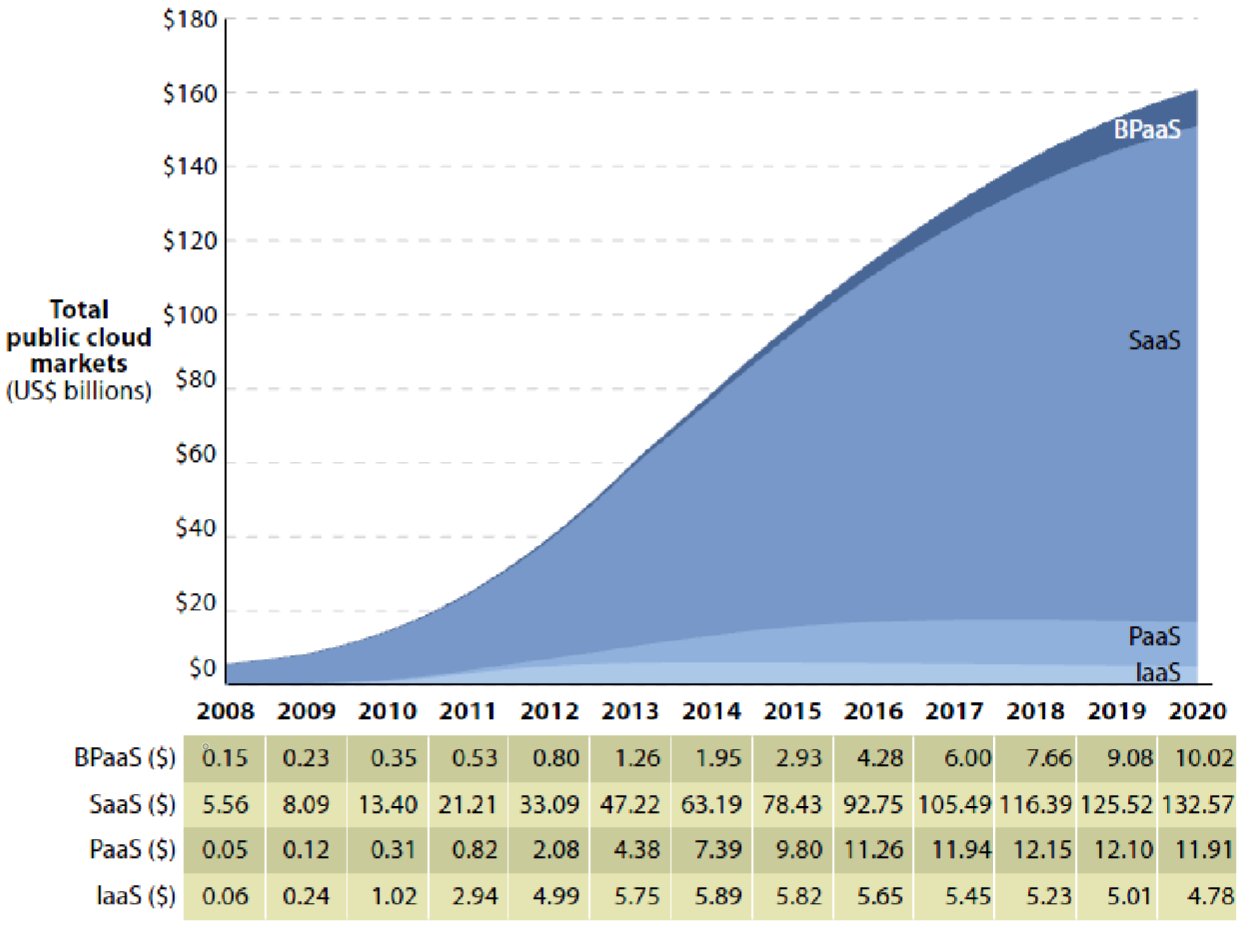
\includegraphics[width=0.7\linewidth]{images/tempsnip4}
    	\caption{Prévisions de la taille du marché du cloud computing  public (Ried, 2011).}
    	\label{fig:tempsnip4}
    \end{figure}
\subsubsection{Vers une définition du cloud computing }
Beaucoup de chercheurs ont tenté de définir le cloud computing (Geelan, 2008 ; McFedries, 2008 ; Buyya, 2009 ; Armbrust, 2010). La plupart des définitions attribuées à ce concept semblent se concentrer seulement sur certains aspects technologiques. L'absence d'une définition standard a généré non seulement des exagérations du marché, mais aussi des confusions. Pour cette raison, il y a eu récemment des travaux sur la normalisation de la définition du cloud computing, à l'exemple de Vaquero et coll (Vaquero, 2009) qui ont comparé plus de 20 définitions différentes et ont proposé une définition globale.  En guise de synthèse des différentes propositions données dans la littérature, nous introduisons une définition mixte, qui correspond aux différents types de cloud considérés dans les travaux réalisés dans cette thèse.

  Nous définissons le cloud comme un modèle informatique qui permet d’accéder, d’une façon transparente et à la demande, à un pool de ressources hétérogènes physiques ou virtualisées (serveurs, stockage, applications et services) à travers le réseau. Ces ressources sont délivrées sous forme de services reconfigurables et élastiques, à base d’un modèle de paiement à l’usage, dont les garanties sont offertes par le fournisseur via des contrats de niveau de service (SLA, Service Level Agreement).     
    
    \subsubsection{Caractéristiques principales du cloud computing}
    Le cloud computing  possède les caractéristiques suivantes :
    \begin{itemize}
    	\item 	\textbf{Accès en libre-service à la demande}. Le cloud computing offre des ressources et services aux utilisateurs à la demande. Les services sont fournis de façon automatique, sans nécessiter d’interaction humaine (Mell, 2011). 
    \item	\textbf{Accès réseau universel.}  Les services de cloud computing  sont facilement accessibles au travers du réseau, par le biais de mécanismes standard, qui permettent une utilisation depuis de multiples types de terminaux (par exemple, les ordinateur portables, tablettes, smartphones) (Mell, 2011). 
   \item \textbf{Mutualisation de ressources} (Pooling). Les ressources du cloud peuvent être regroupées pour servir des utilisateurs multiples, pour lesquels des ressources physiques et virtuelles sont automatiquement attribuées (Mell, 2011). En général, les utilisateurs n’ont aucun contrôle ou connaissance sur l’emplacement exact des ressources fournies. Toutefois, ils peuvent imposer de spécifier l’emplacement à un niveau d’abstraction plus haut.
   \item \textbf{Scalabilité et élasticité.} Des ressources supplémentaires peuvent être automatiquement mises à disposition des utilisateurs en cas d’accroissement de la demande (en réponse à l'augmentation des charges des applications) (Geelan, 2008), et peuvent être libérées lorsqu’elles ne sont plus nécessaires. L’utilisateur a l’illusion d’avoir accès à des ressources illimitées à n'importe quel moment, bien que le fournisseur en définisse généralement un seuil (par exemple : 20 instances par zone est le maximum possible pour Amazon EC2).
   \item \textbf{Autonome.} Le cloud computing  est un système autonome et géré de façon transparente pour les utilisateurs. Le matériel, le logiciel et les données au sein du cloud peuvent être 
    	automatiquement reconfigurés, orchestrés et consolidés en une seule image qui sera fournie à l’utilisateur (Wang, 2008).
    	\item \textbf{Paiement à l’usage.} La consommation des ressources dans le cloud s’adapte au plus près aux besoins de l’utilisateur. Le fournisseur est capable de mesurer de façon précise la consommation (en durée et en quantité) des différents services (CPU, stockage, bande passante,…) ; cela lui permettra de facturer l’utilisateur selon sa réelle consommation (Armbrust, 2009). 
    	\item \textbf{Fiabilité et tolérance aux pannes.} Les environnements cloud tirent parti de la redondance intégrée du grand nombre de serveurs qui les composent en permettant des niveaux élevés de disponibilité et de fiabilité pour les applications qui peuvent en bénéficier (Buyya, 2008). 
    	\item \textbf{Garantie QoS.} Les environnements de cloud peuvent garantir la qualité de service pour les utilisateurs, par exemple, la performance du matériel, comme la bande passante du processeur et la taille de la mémoire (Wang, 2008). 
    	\item \textbf{Basé-SLA.} Les clouds sont gérés dynamiquement en fonction des contrats d’accord de niveau de service (SLA) (Buyya, 2008) entre le fournisseur et l’utilisateur. Le SLA définit des politiques, telles que les paramètres de livraison, les niveaux de disponibilité, la maintenabilité, la performance, l'exploitation, ou autres attributs du service, comme la facturation, et même des sanctions en cas de violation du contrat. Le SLA permet de rassurer les utilisateurs dans leur idée de déplacer leurs activités vers le cloud, en fournissant des garanties de QoS. 
    	Après avoir présenté les caractéristiques essentielles d’un service cloud, nous présentons, brièvement, dans la section suivante, quelques technologies connexes aux clouds.
    	
    \end{itemize} 